\section{Final Solution}
Our final AUC score of 0.90918 results from a complex pipeline from raw data to final score.
Every part of that pipe needs to be (sub-)optimal implemented by our team to get the best score at the end.
The first part ``feature design'' is the most important one and needs expertise, experience and of course a bit luck to capture all signals in the data.

We train 64 single models with the 8 different algorithms and different subsets of 7 feature sets.

We trained 15 stage-I ensemble classifiers with different subsets of CV predictions of 64 single classifiers.

At KDD Cup 2015, GBM outperforms other algorithms.  Our top 8 single models as well as top 2 stage-1 ensemble models are trained with GBM.

We trained 2 stage-II ensemble classifiers with different subsets of CV predictions of 15 stage-I ensemble classifiers.

We trained a stage-III ensemble classifier with CV predictions of 5 classifiers: 1 stage-II ensemble, 3 stage-I ensemble, and 1 individual classifiers.

Performance improvement diminishes as we add more ensemble stages.  The stage-1 ensemble improves the CV AUC score by XXXX from 0.906721 to 0.907688.  The stage-2 ensemble improves the CV AUC score by XXXX to 0.907968.  The stage-3 ensemble improves the CV AUC score by XXXX to 0.908194.\\

We choose subsets of predictions from the previous stage for ensemble model training, 
\begin{figure}[t]
  \centering
    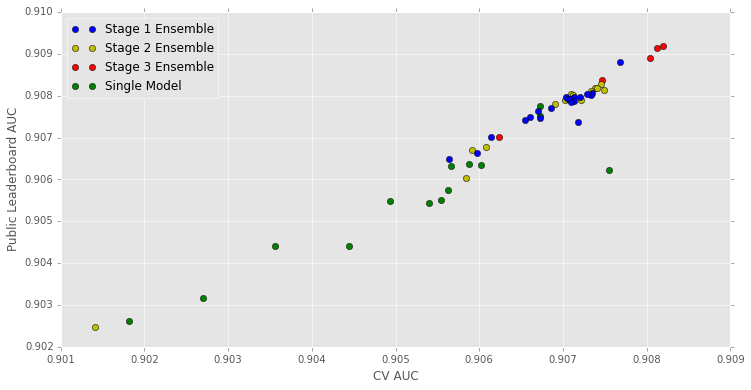
\includegraphics[width=0.5 \textwidth]{cv_lb}
      \caption{5-fold CV vs. public leaderboard AUC scores.}
\end{figure}

A linear combination of the 5 models from table \ref{tb:finalEnsemble} results in train AUC=0.908072 and accuracy=0.887334.
Which leads to 0.90910 public leaderboard score.
By adding 39 courseID correction factors train AUC=0.908194 and public score improved to 0.90918.

\begin{figure*}[!t]
  \centering
    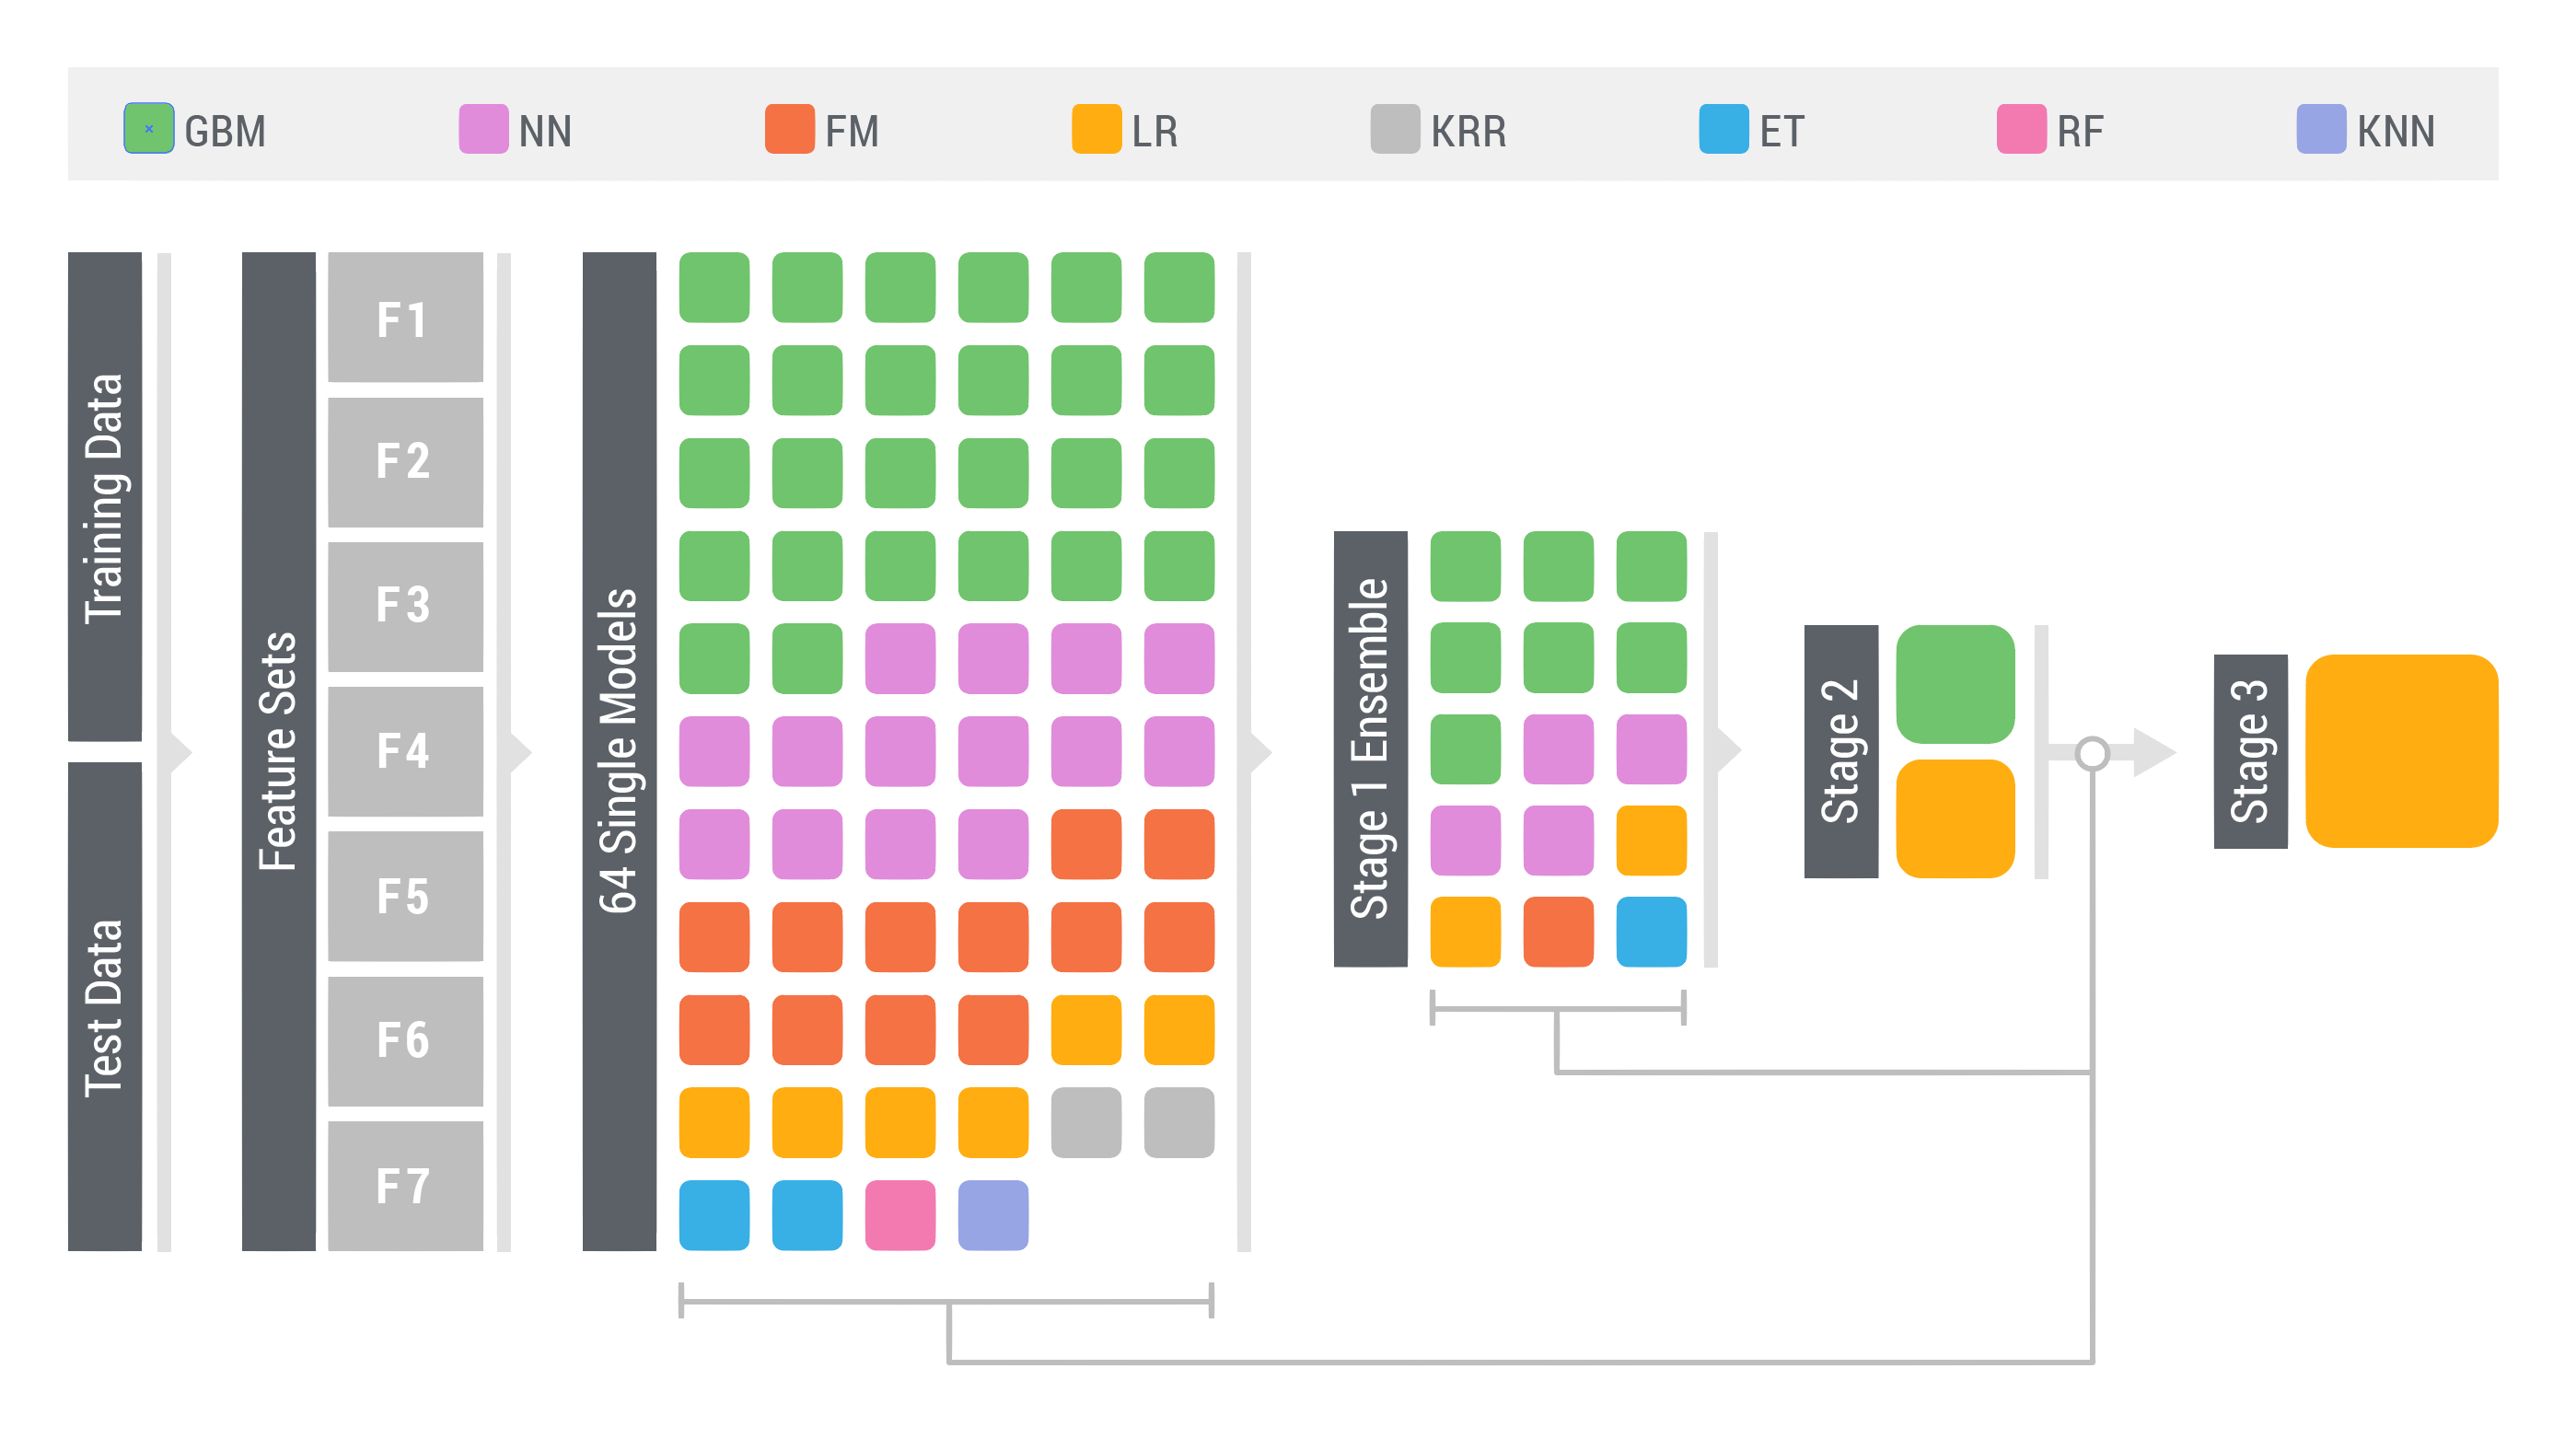
\includegraphics[width=1 \textwidth]{ensemble}
      \caption{End-to-end pipeline for the final solution}
\end{figure*}

\begin{table}
\begin{center}
	\caption{List of models selected in the stage-3 ensemble.}
\begin{tabular}{lllll}
ID 	& Stage 	& Algorithm 	& 5-CV 		& Weight\\ \hline
S1 	& Single	& GBM		& 0.906721 	& 1.1703 \\
E4 	& 1 		& GBM		& 0.907878 	& 1.9626\\
E8 	& 1 		& NN		& 0.907567	& 0.7871\\
E18	& 1		& ET			& 0.906207 	& 0.4580\\
E2	& 2 		& LR			& 0.907968 	& 1.6146\\
\end{tabular}

\label{tb:finalEnsemble}
\end{center}
\end{table}
